% !TEX root = ../Main.tex
\subsection{Freidberg's simple reactor model}
In the \nth{5} chapter of the textbook by Freidberg\cite{freidberg_plasma_2007}, he makes a simple model for designing a fusion reactor power plant.
The model uses simple geometric and electromagnetic assumptions with little involvement of plasma physics. The variables put into the model are shown in \cref{VFR}.
\begin{table}
	\begin{tabular}{lr}
		\toprule
		Symbol                         & Quantity                                                                                 \\
		\midrule
		\(n_\mathrm{flux \ fraction}\) & n flux in breeder end/n flux in breeder start \(\bqty{}\)                                \\
		\(C_F\)                        & Fixed cost propotionality constant \(\bqty{\$}\)                                         \\
		\(C_I\)                        & Nuclear island cost propotionality constant \(\bqty{\$\cdot\si{\watt\per\meter\cubed}}\) \\
		\(P_E\)                        & Desired output power \(\bqty{\si{\mega\watt}}\)                                          \\
		\(P_W\)                        & Maximum wall load \(\bqty{\si{\mega\watt\per\meter\squared}}\)                           \\
		\(B_{\max}\)                   & Magnetic field at the edge of the coil \(\bqty{\si{\tesla}}\)                            \\
		\(\sigma_{\max}\)              & Tensile strenght of the magnetic field coils \(\bqty{\si{\atm}}\)                        \\
		\(\eta_t\)                     & Energy conversion efficiency \(\bqty{}\)                                                 \\
		\bottomrule
	\end{tabular}
	\caption{Variables in the Freidberg's model}
	\label{VFR}
\end{table}
\cref{QFR} shows the output quantities from the model.
\begin{table}
	\begin{tabular}{llr}
		\toprule
		Symbol                    & Quantity                                                       & Obtained values                  \\
		\midrule
		\(b\)                     & Blanket-and-shield thickness                                   & \SI{1.2037}{\meter}              \\
		\(c\)                     & Magnet coil thickness                                          & \SI{0.7993}{\meter}              \\
		\(a\)                     & Minor radius                                                   & \SI{2.0098}{\meter}              \\
		\(R_0\)                   & Major radius                                                   & \SI{4.9583}{\meter}              \\
		\(A\)                     & Aspect ratio                                                   & 2.4670                           \\
		\(A_p\)                   & Plasma surface                                                 & \SI{393.4152}{\meter\squared}    \\
		\(V_p\)                   & Plasma volume                                                  & \SI{395.3509}{\meter\cubed}      \\
		\(P_\mathrm{dens}\)       & Power density                                                  & \SI{4.9685e06}{\watt\per\meter}  \\
		\(p\)                     & Plasma pressure                                                & \SI{7.3672e05}{\pascal}          \\
		\(n\)                     & Particle density                                               & \SI{1.5327e20}{\per\meter\cubed} \\
		\(B_0\)                   & Magnetic field at magnetic axis                                & \SI{4.5744}{\tesla}              \\
		\(\beta\)                 & Normalised plasma pressure                                     & 8.85\%                           \\
		\(\tau_{E_\mathrm{min}}\) & Min confinement time for \(\pqty{p\times\tau_E}_\mathrm{min}\) & \SI{1.1415}{\second}             \\
		\bottomrule
	\end{tabular}
	\caption{Output quantities in the model in Freidberg's\cite{freidberg_plasma_2007} along with the obtained values when inserting the parameters from \cref{Inputparam}}
	\label{QFR}
\end{table}
This model has been implemented in a matlab script provided for the course. The script is shown included in \cref{tokamakDTU_asign_1}.
As an example, the model is run with the following parameters:
\begin{alignat}{3}
	n_\mathrm{flux \ fraction} & = 0.01                                 & \quad P_E      & = \SI{1000}{\mega\watt} \nonumber       \\
	P_W                        & = \SI{4}{\mega\watt\per\meter\squared} & \quad B_{\max} & = \SI{13}{\tesla}    \label{Inputparam} \\
	\sigma_{\max}              & = \SI{3000}{\atm}                      & \quad \eta_t   & = 0.4 \nonumber
\end{alignat}
Note that \(C_F\) and \(C_I\) has been ommited as these serve no purpose for this assignment. It is not of interest how expensive the plant will be. Rather the geometries and physical quantities are of interest.
The results from the model is given in \cref{QFR}.
\subsection{Model sensitivity}
At this point Freidberg has provided a model that produce some reasonable results for a powerplant. It could be interesting to see how this model behaves when some vital parameters are changed. In the last section the model used the parameters shown in \cref{Inputparam}. Now the model will be iteratet over variations in the following parameters, while retaining the rest.
The variable parameters are the electric power \(P_E\), the maximum wall loading \(P_W\), the maximum magnetic field \(B_{\max}\) and the maximum stress \(\sigma_{\max}\).
\cref{IterateTokamakDTU} includes the code for iterating the matlab model over various paremeters.
\subsubsection{Change in desired power output.}
For the rise in megawatts produced (\SIrange{500}{1000}{\mega\watt}) there are a linear rise in aspect ratio, major radius, plasma surface and plasma volume. The rest of the parameters where constant except for the magnetic field strenght at the magnetic axis and the normalised plasma pressure. These are shown in \cref{PE}.
\begin{figure}
	\centering
	\begin{subfigure}[b]{.45\textwidth}
		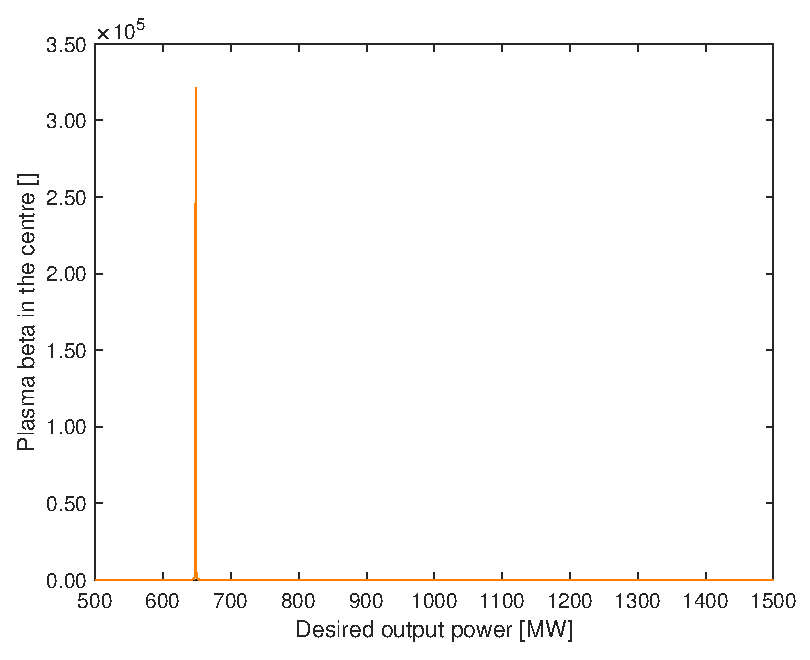
\includegraphics[width=\textwidth]{MatlabFigures/DesiredOutputPower/PlasmaBetaInTheCentre.eps}
		\caption{}
		\label{PEbeta}
	\end{subfigure}
	~
	\begin{subfigure}[b]{.45\textwidth}
		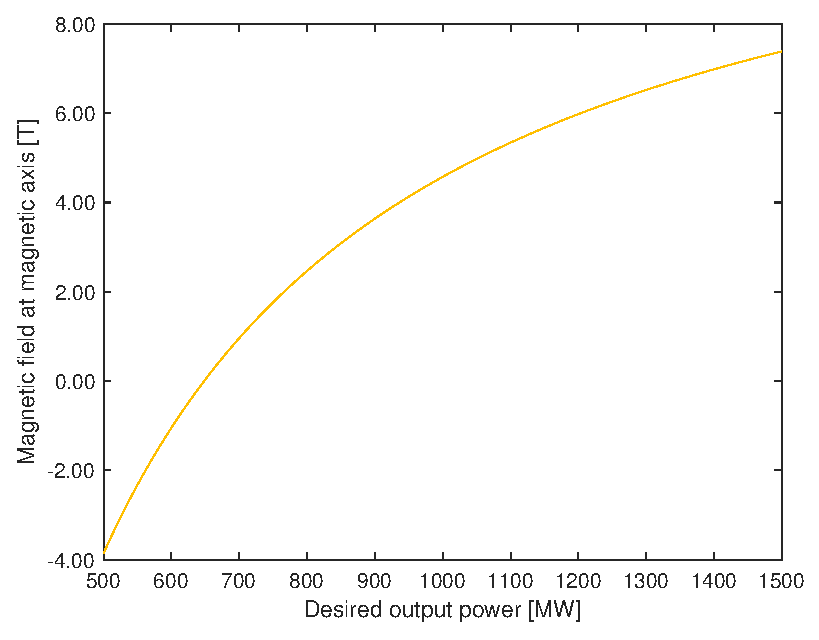
\includegraphics[width=\textwidth]{MatlabFigures/DesiredOutputPower/MagneticFieldAtMagneticAxis.eps}
		\caption{}
		\label{PEmagnet}
	\end{subfigure}
	\caption{The evolution of the normalised plasma pressure (\cref{PEbeta}) and the magnetic field strenght (\cref{PEmagnet}) when changing the desired power output.}
	\label{PE}
\end{figure}
% \subsubsection{\(P_W\) \SIrange{0}{10}{\mega\watt\per\meter\squared}}
% \subsubsection{\(B_{\max}\) \SIrange{0}{20}{\tesla}}
% \subsubsection{\(\sigma_{\max}\) \SIrange{2000}{5000}{\atm}}
\subsection{Elliptic Cross section}
Freidberg's model assumes a circular cross section of the plasma. In reality this is not the case, and as of such we will now make a more realistic, yet still approximate reactor for an elliptic plasma cross section.
In describing the geometry one refers to the elongation ratio:
\begin{align}
	\kappa = \frac{a_{\max}}{a_{\min}}
\end{align}
With $a_{\max}$ the major radius and $a_{\min}$ the minor radius of the ellipse. This parameter ensures a true elliptic cross section as defined by the equation,
\begin{align}
	\frac{x^2}{a_{\max}}+\frac{y^2}{a_{\min}} = 1
\end{align}
which can be parameterised as
\begin{align}
	\mqty[x_1 \\y_1] &= \mqty[a_{\min}\cos{\phi}\\\kappa a_{\min}\sin{\phi}] \\
	\label{eq:inner_ellipse}
\end{align}
\begin{wrapfigure}[14]{r}{.4\textwidth}
	%\vspace{-5mm}
	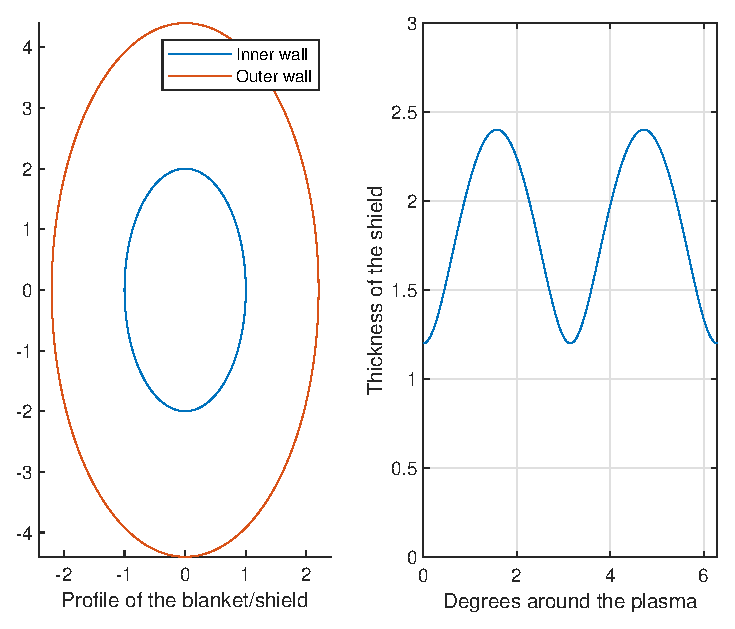
\includegraphics[width=.4\textwidth]{MatlabFigures/ShieldThickness/ShieldThickness.eps}
	\caption{The profile of the blanket-and-shield and the thickness as a function of the angle around origo, \(\phi\).}
	\label{ShTh}
\end{wrapfigure}
Meanwhile the blanket must be implemented as an ellipse or swelled ellipse. The true ellipse results in a difference of thickness in the blanket while the second results in a blanket of equal thickness throughout the structure. To this the choice of implementing the blanket as a true ellipse has been made since it simplifies derivations a bit. Note however that keeping a constant thickness is the preferable option as it will reduce the engineering volume and hence the cost of the machine.\\
The outher layer parameterised is
\begin{align}
    \mqty[x_2 \\y_2] &= \mqty[\pqty{b+a_{\min}}\cos{\phi}\\\kappa \pqty{b+a_{\min}}\sin{\phi}]
    \label{eq:outer_ellipse}
\end{align}
with $b$ the blanket thickness at the minor ellipse axis. Choosing for now, $a_{\min}=2$, $\kappa=2$ and $b=1.2$, \ref{eq:inner_ellipse} and \ref{eq:outer_ellipse} are plotted on Figure \ref{ShTh} along with the variation in thickness of the blanket. \\
Given \ref{eq:inner_ellipse} and \ref{eq:outer_ellipse} the engineering volume can easily be derived if $c\,\cos(\phi)$ and $\kappa\, c\,\sin(\phi)$ is added to the x and y-direction in \ref{eq:outer_ellipse} respectively, where $c$ is the minimum thickness of the magnetic coils that provide the torroidal field. \\
The cross sectional area of an ellipse is $A_{\si{e}}=\pi\, a_{\min}\, a_{\max}$ so the engineered volume becomes
\begin{align}
    V_{\si{I}}=2\,\pi\, R_{0}\,(A_{\si{e,outer}}-A_{\si{e,inner}})=2\,\pi^{2}\, R_{0}\,\left(\left(a_{\min}+b+c\right)^{2}-a_{\min}^{2}\right)\,\kappa
    \label{eq:engineered_volume}
\end{align}
and the plasma volume is similarly calculated as $V_{si{p}}=2\,\pi^2\, R_{0}\, a_{\min}\, a_{\max}$. The plasma surface area is a bit more tricky but the result is
\begin{align}
    S_{\si{p}}=2\,\pi\, R_{0}\, C_{\s{p}}=2\,\pi\, R_{0}\, 4\, a_{\min}\,\int_{0}^{2\,\pi}\sqrt{1-(1-\kappa^{-2})^{1/2}\sin^{2}{\phi}} \, d\si{\phi}
\end{align}
where the integral can be approximated after choosing $\kappa$. Thus our choice of $\kappa$ yields $S_{\si{p}}\approx 8\,\pi\, R_{0}\,a_{\min}\cross 4.8$. The rest of the parameters in the code except $c$ is approximated to be unchanged. Now c is also approximated, or rather overestimated using a slight change to eq. (5.24) in the textbook. The change is that since the force grows with $a_{\min}$ inserting $\kappa\, a_{\min}$ instead yields an overestimation on the vertical force on the magnet. The tensile forces are the same, so the force balance leads to 
\begin{align}
    c=\frac{2\,\xi}{1-\xi}(\kappa\, a+b)
\end{align}
with $\xi=B_{si{c}}^2/4\,\mu_{0}\,\sigma_{\si{max}}$. These new parameter equations are inserted in the code. The parameters that changed significantly are displayed in \ref{tab:ellip_output}. The most dramatic change is the plasma volume and surface area which increased by a factor of around 2 and 3 respectively, this makes sence as the plasma was made twice as high. The coil thickness was also changed significantly due to the overestimation while the rest of the parameters did not change much. This most likely means that the model needs more work to make the approximations more precise.

\begin{table}
	\begin{tabular}{llr}
		\toprule
		Symbol                    & Quantity                                                       & Obtained values                  \\
		\midrule
		
		\(c\)                     & Magnet coil thickness                                          & \SI{1.30}{\meter}              \\
		\(A_p\)                   & Plasma surface                                                 & \SI{1206}{\meter\squared}    \\
		\(V_p\)                   & Plasma volume                                                  & \SI{793}{\meter\cubed}      \\
		\(P_\mathrm{dens}\)       & Power density                                                  & \SI{2.48e06}{\watt\per\meter}  \\
		\(p\)                     & Plasma pressure                                                & \SI{5.20e05}{\pascal}          \\
		\(n\)                     & Particle density                                               & \SI{1.08e20}{\per\meter\cubed} \\
		\(\beta\)                 & Normalised plasma pressure                                     & 6.17\%                           \\
		\(\tau_{E_\mathrm{min}}\) & Min confinement time for \(\pqty{p\times\tau_E}_\mathrm{min}\) & \SI{1.62}{\second}             \\
		\bottomrule
	\end{tabular}
	\caption{Output quantities from the elliptical model}
	\label{tab:ellip_output}
\end{table}

\subsection{Main parameters for DEMO}

Setting $P_{\si{E}}=2000$ in the elliptical model yields the output parameters seen in table \ref{tab:DEMO}. Since $R_{0}$ is directly proportional to the electric power this of course increases linearly. The other geometric output parameters regarding areas and volumes  therefore also increases. $\beta$ has decreased a lot, so the plasma is not confined effectively in DEMO.

\begin{table}
	\begin{tabular}{llr}
		\toprule
		Symbol                    & Quantity                                                       & Obtained values                  \\
		\midrule
		\(b\)                     & Blanket-and-shield thickness                                   & \SI{1.20}{\meter}              \\
		\(c\)                     & Magnet coil thickness                                          & \SI{1.30}{\meter}              \\
		\(a\)                     & Minor radius                                                   & \SI{2.01}{\meter}              \\
		\(R_0\)                   & Major radius                                                   & \SI{9.95}{\meter}              \\
		\(A\)                     & Aspect ratio                                                   & 4.95                          \\
		\(A_p\)                   & Plasma surface                                                 & \SI{2.41e03}{\meter\squared}    \\
		\(V_p\)                   & Plasma volume                                                  & \SI{1.59e03}{\meter\cubed}      \\
		\(P_\mathrm{dens}\)       & Power density                                                  & \SI{2.48e06}{\watt\per\meter}  \\
		\(p\)                     & Plasma pressure                                                & \SI{5.20e05}{\pascal}          \\
		\(n\)                     & Particle density                                               & \SI{1.08e20}{\per\meter\cubed} \\
		\(B_0\)                   & Magnetic field at magnetic axis                                & \SI{8.80}{\tesla}              \\
		\(\beta\)                 & Normalised plasma pressure                                     & 1.69\%                           \\
		\(\tau_{E_\mathrm{min}}\) & Min confinement time for \(\pqty{p\times\tau_E}_\mathrm{min}\) & \SI{1.62}{\second}             \\
		\bottomrule
	\end{tabular}
	\caption{Output quantities for DEMO using the elliptical model with $P_{si{E}}=2$}
	\label{tab:DEMO}
\end{table}

\subsection{Designs for DEMO}

With $\kappa=2$ and $A=R_{0}/a_{\min}=3\Leftrightarrow R_{0}=3\, a_{\min}$ $A$ is changed from 4.95 to 3 when going from Friedberg's model to this model. Meanwhile these changes yields the parameters seen in table \ref{tab:DEMO2}. Besides the obvious geometric changes which has decreased due to decreasing $R_{0}$. The pressure has increased while the magnetic field has decreased. Therefor a better confinement is achieved since this increases $\beta$. This is a positive, and decreasing the aspect ratio a bit is therefore recommended. Additional time could be spend on optimising this, but we are unfortunately unable to do so due to time and space restrictions.

\begin{table}
	\begin{tabular}{llr}
		\toprule
		Symbol                    & Quantity                                                       & Obtained values                  \\
		\midrule
		\(b\)                     & Blanket-and-shield thickness                                   & \SI{1.20}{\meter}              \\
		\(c\)                     & Magnet coil thickness                                          & \SI{1.30}{\meter}              \\
		\(a\)                     & Minor radius                                                   & \SI{2.01}{\meter}              \\
		\(R_0\)                   & Major radius                                                   & \SI{6.03}{\meter}              \\
		\(A\)                     & Aspect ratio                                                   & 3                          \\
		\(A_p\)                   & Plasma surface                                                 & \SI{1.46e03}{\meter\squared}    \\
		\(V_p\)                   & Plasma volume                                                  & \SI{962}{\meter\cubed}      \\
		\(P_\mathrm{dens}\)       & Power density                                                  & \SI{4.01e06}{\watt\per\meter}  \\
		\(p\)                     & Plasma pressure                                                & \SI{6.68e05}{\pascal}          \\
		\(n\)                     & Particle density                                               & \SI{1.39e20}{\per\meter\cubed} \\
		\(B_0\)                   & Magnetic field at magnetic axis                                & \SI{6.07}{\tesla}              \\
		\(\beta\)                 & Normalised plasma pressure                                     & 4.55\%                           \\
		\(\tau_{E_\mathrm{min}}\) & Min confinement time for \(\pqty{p\times\tau_E}_\mathrm{min}\) & \SI{1.26}{\second}             \\
		\bottomrule
	\end{tabular}
	\caption{Output quantities for DEMO using the elliptical model with $P_{si{E}}=2$, $\kappa=2$ and setting $A=3$}
	\label{tab:DEMO2}
\end{table}

\subsection{$A$ and $\kappa$ as free parameters}

For this assignment we have chosen to try and optimise $\beta$ and $V_{\si{I}}$ with $A$ and $\kappa$ as free parameters. $\beta$ is optimised first. The magnetic field in the centre was approximated as
\begin{align}
    B_{0}=\frac{R_{0}-a-b}{R_{0}}\,B_{\max}=(1-\frac{1}{A}-\frac{A\, b}{a_{\min}})\, B_{\max}
\end{align}
this yields 
\begin{align}
    \beta=\frac{2\, p\mu_{0}}{(1-\frac{1}{A}-\frac{A\, b}{a_{\min}})^{2}}
\end{align}
Differentiating with respect to $A$, setting the expression equal to zero and solving for $A$ yields $A=\sqrt{a/b}=\R_{0}/a_{\min}\Leftrightarrow R_{0}=\sqrt{a^{3}/b}$. Meanwhile inserting this expression into eq. 
\ref{eq:engineered_volume}, substituting $a_{min}=a_{\max}/\kappa$,
differentiating with respect to $\kappa$, setting the expression equal to zero and solving yields $a_{\max}=-(b+c)\,\kappa/6$ so $a_{\min}=-(b+c)/6$. Next Freidberg's expression for $c$ is inserted and we solve for $\kappa$ which yields
\begin{align}
    \kappa=\frac{6\, a_{\min}\,\xi-b\,\xi-6\, a_{\min}-b}{2\,a_{\min}\,\xi}
\end{align}
$\kappa$ must of course be positive(as must the expression for $a_{\min}$) so it really must be the size of this expression that is calculated. This is inserted into the code yielding the output parameters seen in table \ref{tab:DEMO3}. While an extremely large $\beta$ and a very small engineered volume is achieved, there is most likely other problems with this design.
\begin{table}
	\begin{tabular}{llr}
		\toprule
		Symbol                    & Quantity                                                       & Obtained values                  \\
		\midrule
		\(b\)                     & Blanket-and-shield thickness                                   & \SI{1.20}{\meter}              \\
		\(c\)                     & Magnet coil thickness                                          & \SI{1.30}{\meter}              \\
		\(a\)                     & Minor radius                                                   & \SI{2.01}{\meter}              \\
		\(R_0\)                   & Major radius                                                   & \SI{2.60}{\meter}              \\
		\(A\)                     & Aspect ratio                                                   & 1.29                          \\
		\(A_p\)                   & Plasma surface                                                 & \SI{630}{\meter\squared}    \\
		\(V_p\)                   & Plasma volume                                                  & \SI{414}{\meter\cubed}      \\
		\(P_\mathrm{dens}\)       & Power density                                                  & \SI{9.49e06}{\watt\per\meter}  \\
		\(p\)                     & Plasma pressure                                                & \SI{1.02e05}{\pascal}          \\
		\(n\)                     & Particle density                                               & \SI{2.12e20}{\per\meter\cubed} \\
		\(B_0\)                   & Magnetic field at magnetic axis                                & \SI{-3.09}{\tesla}              \\
		\(\beta\)                 & Normalised plasma pressure                                     & 26.9\%                           \\
		\(\tau_{E_\mathrm{min}}\) & Min confinement time for \(\pqty{p\times\tau_E}_\mathrm{min}\) & \SI{1.26}{\second}             \\
		\bottomrule
	\end{tabular}
	\caption{Output quantities for the elliptical model after $\beta$ and $A$ has been optimised}
	\label{tab:DEMO3}
\end{table}







%, even after increasing the radii to accomodate the larger ellipses describing the blanket-and-shield. This does however mean that the fixed thickness, \(b\) from Freidberg's model is variable. To find this variation the parametric ellipses defining the blanket-and-shield are defined with \(b\) being the length difference between the larger radii and the length difference between the smaller radii.
%\begin{wrapfigure}[14]{r}{.4\textwidth}
	%\vspace{-5mm}
%	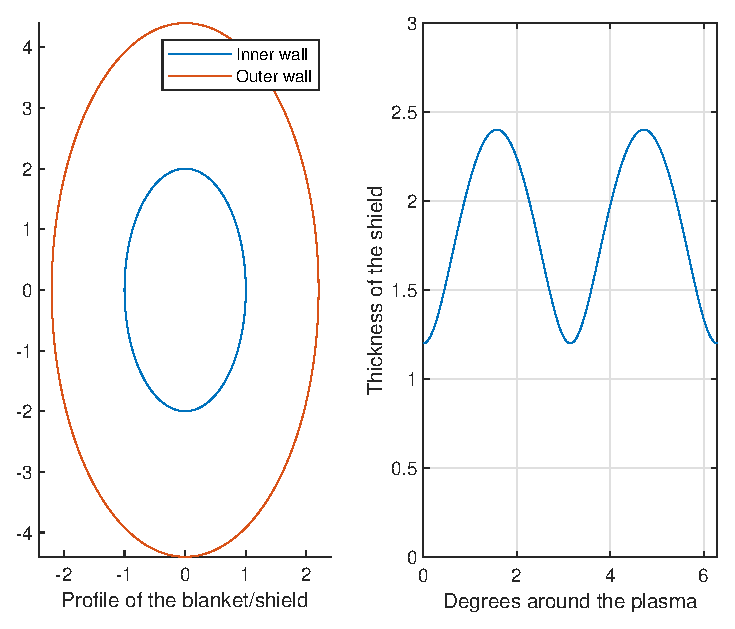
\includegraphics[width=.4\textwidth]{MatlabFigures/ShieldThickness/ShieldThickness.eps}
%	\caption{The profile of the blanket-and-shield and the thickness as a function of the angle around origo, \(\phi\). The parameters here are given in \cref{ellparam}}
%	\label{ShTh}
%\end{wrapfigure}
%\begin{align}
%	\mqty[x_1 \\y_1] &= \mqty[a_{\min}\cos{\phi}\\\kappa a_{\min}\sin{\phi}] \\
%	\mqty[x_2 \\y_2] &= \mqty[\pqty{b+a_{\min}}\cos{\phi}\\\kappa \pqty{b+a_{\min}}\sin{\phi}]
%\end{align}
%At a given angle, \(\phi\), the distance must be:
%\begin{align}
%	\vb{u}-\vb{v}       & = \mqty[\cos{\phi}b                                  \\\kappa\sin{\phi}b] \\
%	\abs{\vb{u}-\vb{v}} & = \sqrt{\cos^2{\phi}\ b^2+\kappa^2\sin^2{\phi}\ b^2}
%\end{align}
%An example is given in \cref{ShTh}. Here the parameters are:
%\begin{alignat}{3}\label{ellparam}
%	\mqty{a_{\min} \\\kappa\\b}&\ \mqty{=\\=\\=}\ &\mqty{2\\2\\1.2}
%\end{alignat}
